\subsection{Concordia Contracts Provider} \label{subsection:4-3-5-concordia-contracts-provider-service}

\subsubsection{Περιγραφή - Στόχοι υπηρεσίας}

Η υπηρεσία Contracts Provider αποτελεί μία βοηθητική υπηρεσία η οποία υλοποιεί ένα απλό αποθετήριο για τα contract artifacts. Είναι γραμμένη σε JavaScript και διαθέτει δύο HTTP \textenglish{endpoints}, ένα για τη μεταφόρτωση (upload) των artifacts προς την υπηρεσία και ένα για τη λήψη (download) από την υπηρεσία. Η υπηρεσία υποστηρίζει επίσης την επισύναψη ετικετών στα artifacts, όπως η έκδοση (version) ή το κλαδί ανάπτυξης (branch, για παράδειγμα \textenglish{master/develop}). Η αρχιτεκτονική της υπηρεσίας φαίνεται το σχήμα \ref{figure:4-3-concordia-contracts-provider-architecture}.

\begin{figure}[H]
    \centering
    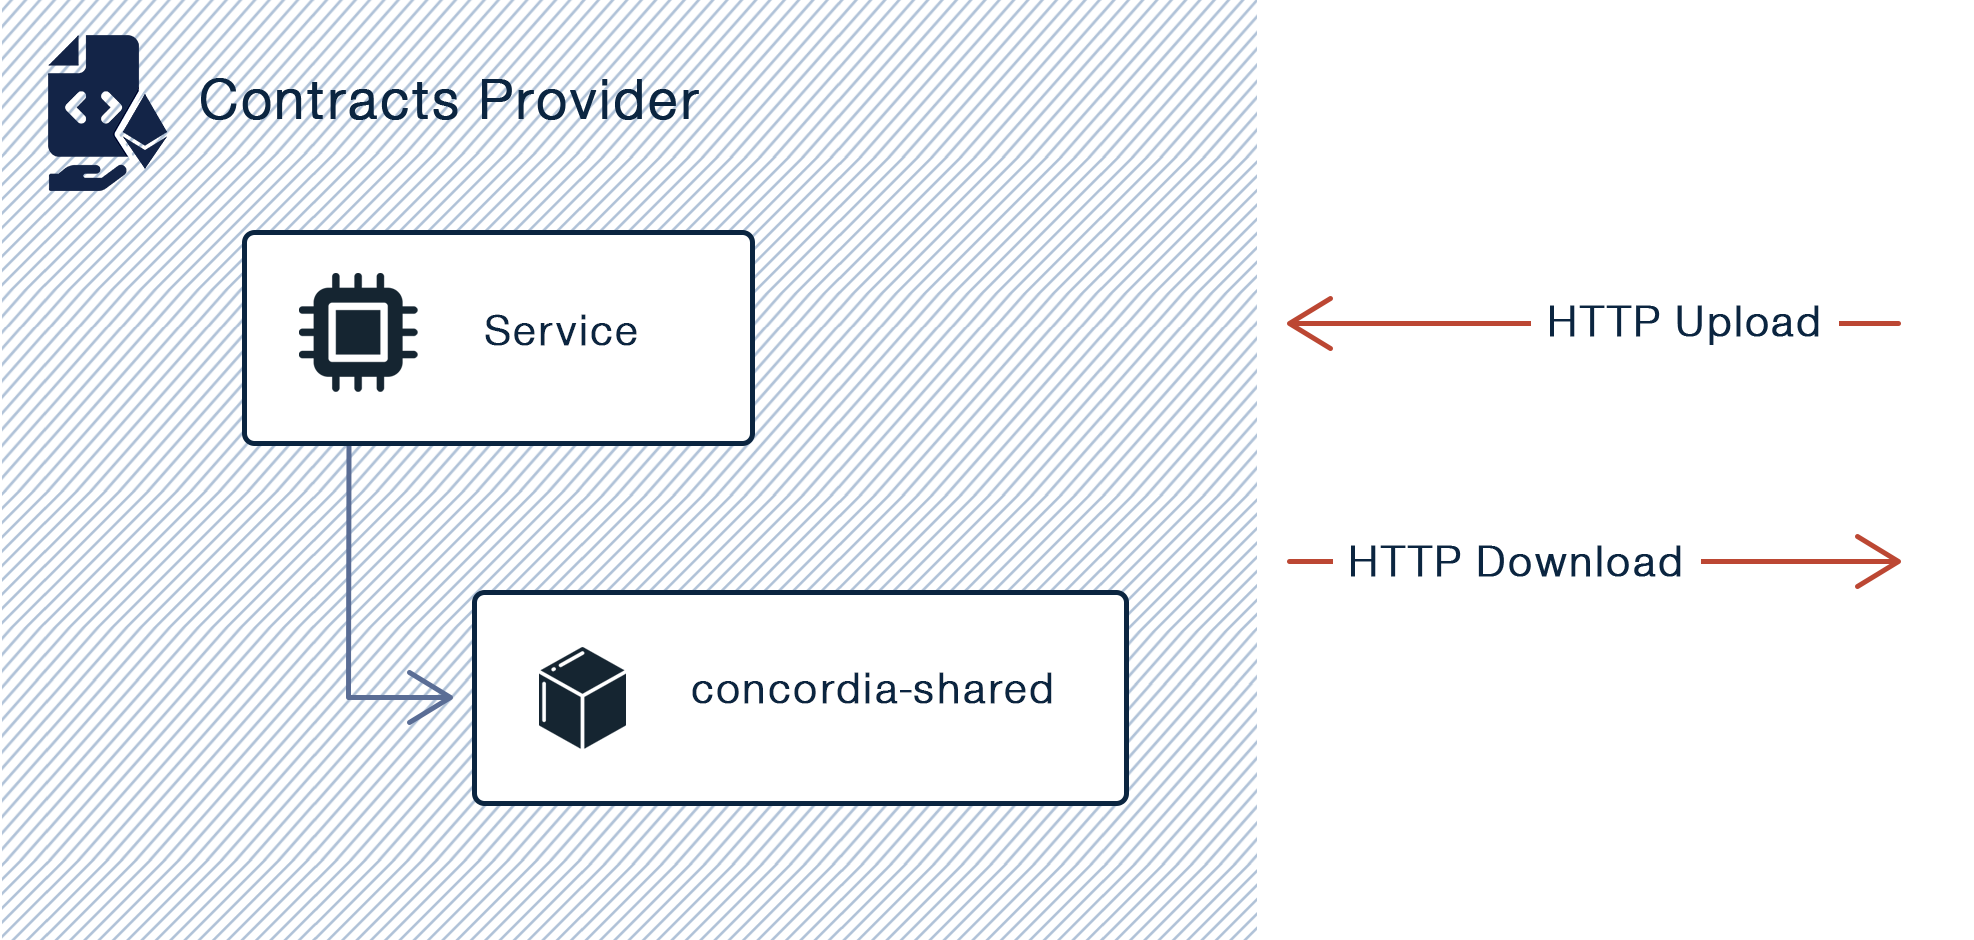
\includegraphics[width=.6\textwidth]{assets/figures/chapter-4/4.3.architecture-4.3.5.concordia-contracts-provider-architecture}
    \caption{Αρχιτεκτονική υπηρεσίας Concordia Contracts Provider}
    \label{figure:4-3-concordia-contracts-provider-architecture}
\end{figure}

Η υπηρεσία χρησιμοποιείται σε μία προσπάθεια αποσύνδεσης της βασικής εφαρμογής που υλοποιεί η υπηρεσία Concordia Application από μία συγκεκριμένη έκδοση των contracts. Οι λόγοι που αυτό είναι επιθυμητό αναπτύχθηκαν στην περιγραφή της υπηρεσίας Concordia \textenglish{Application} (υποενότητα \ref{subsection:4-3-2-concordia-application-service}). Ωστόσο, η υπηρεσία Contracts Provider αποτελεί σημείο κεντροποίησης του συστήματος, για το λόγο αυτό θεωρείται προσωρινή λύση η οποία θα μπορούσε να αντικατασταθεί από αποκεντρωτικές λύσεις όπως η μεταφόρτωση των artifacts στο IPFS και ο διαμοιρασμός τους από εκεί.

\subsubsection{Διανομή}

Η υπηρεσία αυτή γίνεται διαθέσιμη για χρήση ως docker image μέσω του αποθετηρίου εικόνων dockerhub. Οι χρήστες μπορούν χρησιμοποιώντας μεταβλητές περιβάλλοντος να αλλάξουν παραμέτρους της εκτέλεσης, όπως τη διαδρομή αποθήκευσης των μεταφορτωμένων contract artifacts.